\section{TEST OF GHOST BUSTER ALGORITHM}

During the step of muon track reconstruction it is common that one physical muon causes a few muon candidates with similar track parameters. The additional candidates are often called \textit{ghosts}. The step of eliminating \textit{ghosts} is called Ghost-Buster. Ghost-Buster takes the input set of muon candidates and produces the output set of selected candidates. The algorithm of Ghost-Buster is based on comparing azimuthal angle of muon candidates. Sometimes two or more physical muons appear in Overlap region per one event. Well working Ghost-Buster is expected to select the same number of muon candidates as the number of physical muons. For the present article performance of Ghost-Buster emulator was studied.

In the beginning the input set of candidates is taken and they are sorted by quality. Then all candidates are checked in a loop whether their azimuthal angle is close to the azimuthal angle of candidates which are already in the output set (that is performed in a nested loop). If the angle difference is smaller than veto \textit{window} (set to 5$^\circ$) then the candidate from the input set is recognised as a \textit{ghost} and is not passed to the output set. Consequently input candidate with the best quality is always forwarded to the output set.

Chance for finding and eliminating \textit{ghosts} successfully depends significantly on the width of the veto \textit{window}. To study this dependency data samples with simulated single muon events were used. In the Fig. \ref{prob_vs_phi} there is a plot of probability of getting certain number of candidates at the Ghost-Buster output set with respect to veto \textit{window} width. This plot was done for events with both generated muons propagating into the whole Overlap region, that is with pseudorapidity $0.83 < \eta < 1.24$.
\begin{figure}[t]
\centering
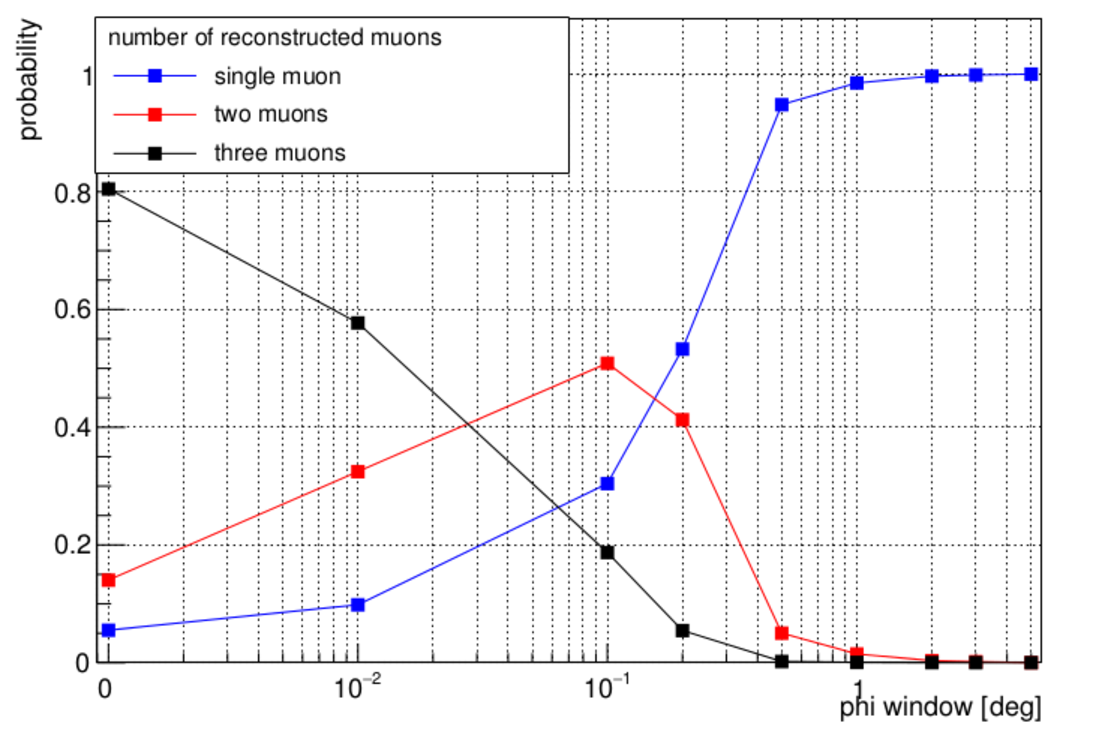
\includegraphics[width=0.7\textwidth]{prob_phi.pdf}
\caption{Results obtained for sample with single muon events. Probability of multiple muon reconstruction on the output of Ghost-Buster vs $\phi$ \textit{window} width. Points on the left edge of plot refer to \textit{window} width set to 0$^\circ$. }
\label{prob_vs_phi}
\end{figure} 
For the very small values of veto \textit{window} width Ghost-Buster's performance is degenerated - in most cases single physical muon will be reconstructed as multiple candidates. For 0.5$^\circ$\textrm{ }and 1$^\circ$\textrm{ }Ghost-Buster is clearly much more effective and for 5$^\circ$\textrm{ }probability of receiving single candidate on the output set is bigger than 99.9\%. 

Good \textit{ghosts} selection has however its price. For high transverse momenta Ghost-Buster decreases efficiency of the $\mu^{+}\mu^{-}$ pairs reconstruction. This effect was studied on data samples with simulated single J/$\Psi \rightarrow \mu^{+}\mu^{-}$ decay events. In the Fig. \ref{divmom} there is a plot of efficiency of the $\mu^{+}\mu^{-}$ pairs reconstruction vs J/$\psi$ generated transverse momentum. This plot was done for events with both generated muons propagating into the middle Overlap region, that is with pseudorapidity $0.9 < \eta < 1.15$. For J/$\psi$ transverse momentum bigger than 40 GeV/c efficiency drops from $(92.4\pm0.5)\%$ (when cut on azimuthal angle is disabled) to $(86.2\pm0.6)\%$ (when 5$^\circ$\textrm{ }cut is used). This is a consequence of fact that for high J/$\psi$ momenta the decay resulting in muons propagating into narrow $\phi$ \textit{window} is more probable.
\begin{figure}[t]
\centering
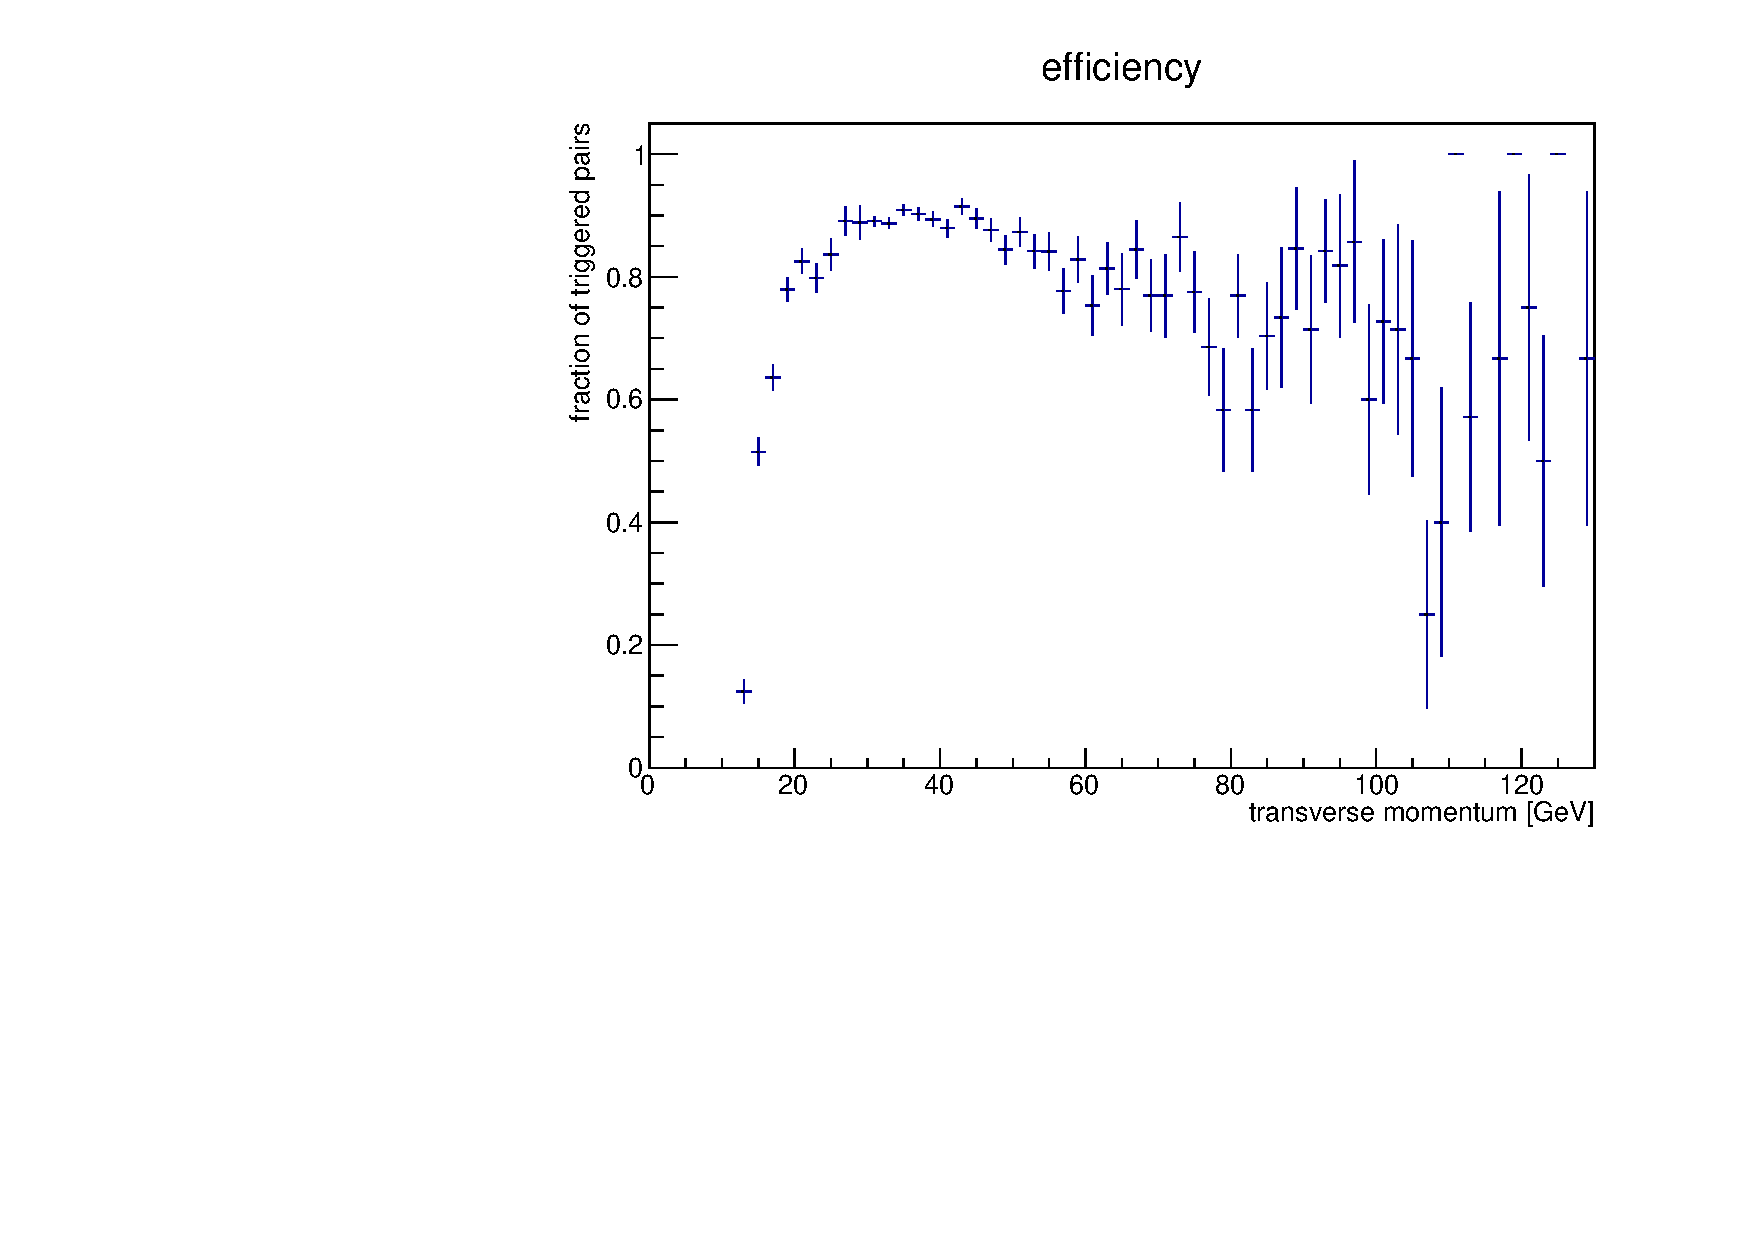
\includegraphics[width=0.7\textwidth]{efficiency_GB_5.pdf}
\caption{Efficiency of reconstructing two muon candidates vs J/$\psi$ transverse momentum.}
\label{divmom}
\end{figure} 
